\documentclass{article}

\usepackage[final]{neurips_2023}

\usepackage[utf8]{inputenc}
\usepackage[T1]{fontenc}
\usepackage{amsmath,amssymb,amsfonts}
\usepackage{graphicx}
\usepackage{booktabs}
\usepackage{hyperref}
\usepackage{xcolor}
\usepackage{multirow}
\usepackage{subcaption}
\usepackage{microtype}

\graphicspath{{./Figures/}{./figures/}{./}}

\title{Geometric Universality is Objective-Contingent: \\
Testing the Platonic Representation Hypothesis \\
Across Language and Vision-Language Models}

\author{
  Gyeongbin Ryoo\\
  Dartmouth College\\
  \texttt{gyeongbin.ryoo.gr@dartmouth.edu}
}

\begin{document}

\maketitle

\begin{abstract}
The Platonic Representation Hypothesis posits that neural networks converge toward shared geometric representations as they scale. We conduct a systematic empirical investigation across ten language and vision-language models using fifteen experiments and six geometric metrics. Our analysis reveals that geometric convergence is strongly contingent on training objective: models sharing the same objective exhibit high alignment (CKA $> 0.75$) regardless of architecture, while cross-objective alignment remains weak (CKA $\approx 0.18$). We uncover a critical methodological insight---CLIP requires end-of-sequence rather than classification token pooling, resolving a 3,500$\times$ discrepancy in reported alignment. Trained structural probes reveal syntactic structure invisible to raw correlations ($\rho$: 0.02 $\rightarrow$ 0.53), and geometric similarity predicts downstream task agreement ($\rho = -0.77$). These findings refine the Platonic hypothesis: neural networks converge toward \emph{objective-specific} representations rather than a universal shared structure. Code is available at \url{https://github.com/growingpenguin/cross-model-neighborhood-consistency}.
\end{abstract}

\section{Introduction}

Neural networks trained on different data, with different architectures, and for different tasks can nonetheless arrive at strikingly similar internal representations. This observation lies at the heart of the Platonic Representation Hypothesis, recently articulated by Huh et al.~\cite{huh2024platonic}. If true, this hypothesis would suggest that learned representations reflect deep regularities in the data-generating process itself, not merely the inductive biases of individual models. The implications would be profound: transfer learning would work because models converge to shared solutions, interpretability tools developed for one architecture might transfer to others, and the apparent diversity of neural network designs might mask an underlying unity in what they learn.

Evidence for representational convergence has accumulated across several research threads. Hewitt and Manning~\cite{hewitt2019structural} demonstrated that BERT encodes syntactic parse trees as metric distances in a linearly-accessible subspace, achieving Spearman correlations exceeding 0.8 with gold-standard parse tree distances. Coenen et al.~\cite{coenen2019visualizing} showed that syntax and semantics occupy geometrically separable regions within BERT's representation space, with different attention heads specializing in different linguistic phenomena. In the vision domain, Raghu et al.~\cite{raghu2021vision} found that vision transformers and CNNs converge toward increasingly similar representations as model capacity increases, despite their fundamentally different inductive biases.

However, recent work complicates this narrative. Studies on multimodal learning~\cite{emergence2024multimodal} have shown that alignment depends critically on information redundancy between modalities and can even be detrimental when modalities carry complementary information. This raises a fundamental question: under what conditions does representational convergence actually occur?

We address this question through a comprehensive empirical study spanning ten models, fifteen experiments, and six geometric metrics. Our investigation yields four key findings. First, we establish that training objective---not architecture, scale, or training data---is the primary determinant of geometric structure. Second, we identify a critical methodological artifact in prior CLIP analyses: using the wrong pooling token produces near-zero alignment that jumps to 0.74 with correct methodology. Third, we show that syntactic structure is linearly encoded but requires learned projections to access, reconciling apparently conflicting results in the probing literature. Finally, we demonstrate that geometric alignment predicts downstream task performance, establishing practical relevance for these theoretical insights.

\section{Related Work}

The discovery that neural networks encode interpretable structure geometrically has reshaped our understanding of representation learning. Coenen et al.~\cite{coenen2019visualizing} showed that BERT's layers progressively separate syntactic from semantic information in distinct subspaces, with attention heads specializing for different linguistic phenomena. Hewitt and Manning~\cite{hewitt2019structural} formalized these intuitions through structural probes, demonstrating that a learned linear transformation applied to BERT's hidden states recovers parse tree distances with Spearman $\rho > 0.8$. Their depth probe similarly recovers word depth in the parse tree, suggesting that syntax is encoded as geometric structure.

For measuring representational similarity across models, Centered Kernel Alignment (CKA) introduced by Kornblith et al.~\cite{kornblith2019similarity} has emerged as the standard metric. CKA offers several desirable properties: invariance to orthogonal transformations, invariance to isotropic scaling, and the ability to compare representations of different dimensionalities. Raghu et al.~\cite{raghu2021vision} applied CKA systematically to vision models, showing that vision transformers and CNNs learn increasingly similar representations as they scale, despite their different architectural inductive biases.

The Platonic Representation Hypothesis, articulated by Huh et al.~\cite{huh2024platonic}, synthesizes these findings into a bold claim: capable neural networks converge toward a shared ``Platonic'' representation of reality regardless of their architecture or training modality. Their evidence focused primarily on increasing vision-language alignment with scale. Our work provides the first systematic test of this hypothesis across multiple architectures and training objectives, revealing that the conditions for convergence are more nuanced than the original formulation suggests.

\section{Experimental Setup}

\subsection{Models}

Our investigation centers on ten models spanning three architectural families and five training objectives, summarized in Table~\ref{tab:models}. This selection enables several controlled comparisons. BERT and RoBERTa share the masked language modeling objective but differ in training corpus and optimization---comparing them reveals variation within an objective family. GPT-2 and Mistral-7B share autoregressive training but differ by 56$\times$ in scale, allowing us to test whether larger models converge toward representations learned by different objectives. CLIP's text and vision encoders are trained jointly but process different modalities, providing a test case for cross-modal convergence.

\begin{table}[t]
\centering
\caption{Models analyzed in this study, grouped by training objective.}
\label{tab:models}
\small
\begin{tabular}{@{}llll@{}}
\toprule
\textbf{Model} & \textbf{Architecture} & \textbf{Objective} & \textbf{Parameters} \\
\midrule
BERT & Transformer Encoder & Masked LM & 110M \\
RoBERTa & Transformer Encoder & Masked LM & 125M \\
DistilBERT & Transformer Encoder & Knowledge Distillation & 66M \\
ALBERT & Transformer Encoder & Masked LM & 12M \\
\midrule
GPT-2 & Transformer Decoder & Autoregressive LM & 124M \\
GPT-2-XL & Transformer Decoder & Autoregressive LM & 1.5B \\
Mistral-7B & Transformer Decoder & Autoregressive LM & 7B \\
\midrule
T5-Encoder & Encoder-Decoder & Span Corruption & 220M \\
CLIP-Text & Transformer Encoder & Contrastive & 63M \\
CLIP-Vision & Vision Transformer & Contrastive & 86M \\
\bottomrule
\end{tabular}
\end{table}

\subsection{Metrics and Data}

To capture different aspects of geometric similarity, we employ six complementary metrics. Centered Kernel Alignment (CKA) measures representation similarity via the Hilbert-Schmidt Independence Criterion, capturing both linear and nonlinear relationships. Procrustes distance quantifies structural similarity under optimal orthogonal transformation. Mutual $k$-NN overlap examines whether models organize examples into similar local neighborhoods. We also compute Spearman correlation between pairwise distance matrices, and measure clustering agreement via Adjusted Rand Index (ARI) and Normalized Mutual Information (NMI).

Our evaluation spans four datasets: WikiText-2 (1,000 sentences) for general language analysis, COCO Captions (1,000 image descriptions) for vision-language comparisons, CIFAR-10 (200 images with generated captions) for cross-modal analysis, and SST-2 (2,000 sentences) for downstream sentiment classification. We extract representations from the residual stream using CLS token pooling for encoders, last token for autoregressive models, and---critically, as we discuss in Section~\ref{sec:clip}---EOS pooling for CLIP.

\subsection{Reproducibility}

All experiments were conducted on Google Colab using a single NVIDIA A100-SXM4-40GB GPU. We extracted representations using batch size 16 with maximum sequence length 256 tokens. For each dataset, we sampled 400 sentences for the main alignment analyses. Representations were extracted from the last hidden state of each layer; for autoregressive models we used last-token pooling, while encoder models used CLS-token pooling. Bootstrap confidence intervals used 100 resampling iterations. Total extraction time across all ten models was approximately 45 minutes. All code is available in our repository.

\section{Results}

\subsection{Training Objective Dominates Geometric Structure}

We begin by computing pairwise alignment across all models using each of our six metrics. Figure~\ref{fig:alignment} reveals a striking pattern: models cluster strongly by training objective rather than by architecture or scale. BERT and RoBERTa, despite their differences in training corpus and optimization, achieve CKA of 0.754. DistilBERT, trained via knowledge distillation from BERT, maintains CKA of 0.72 with its teacher. In contrast, BERT-GPT-2 alignment reaches only 0.182, and BERT-CLIP alignment with CLS pooling approaches zero.

\begin{figure}[t]
\centering
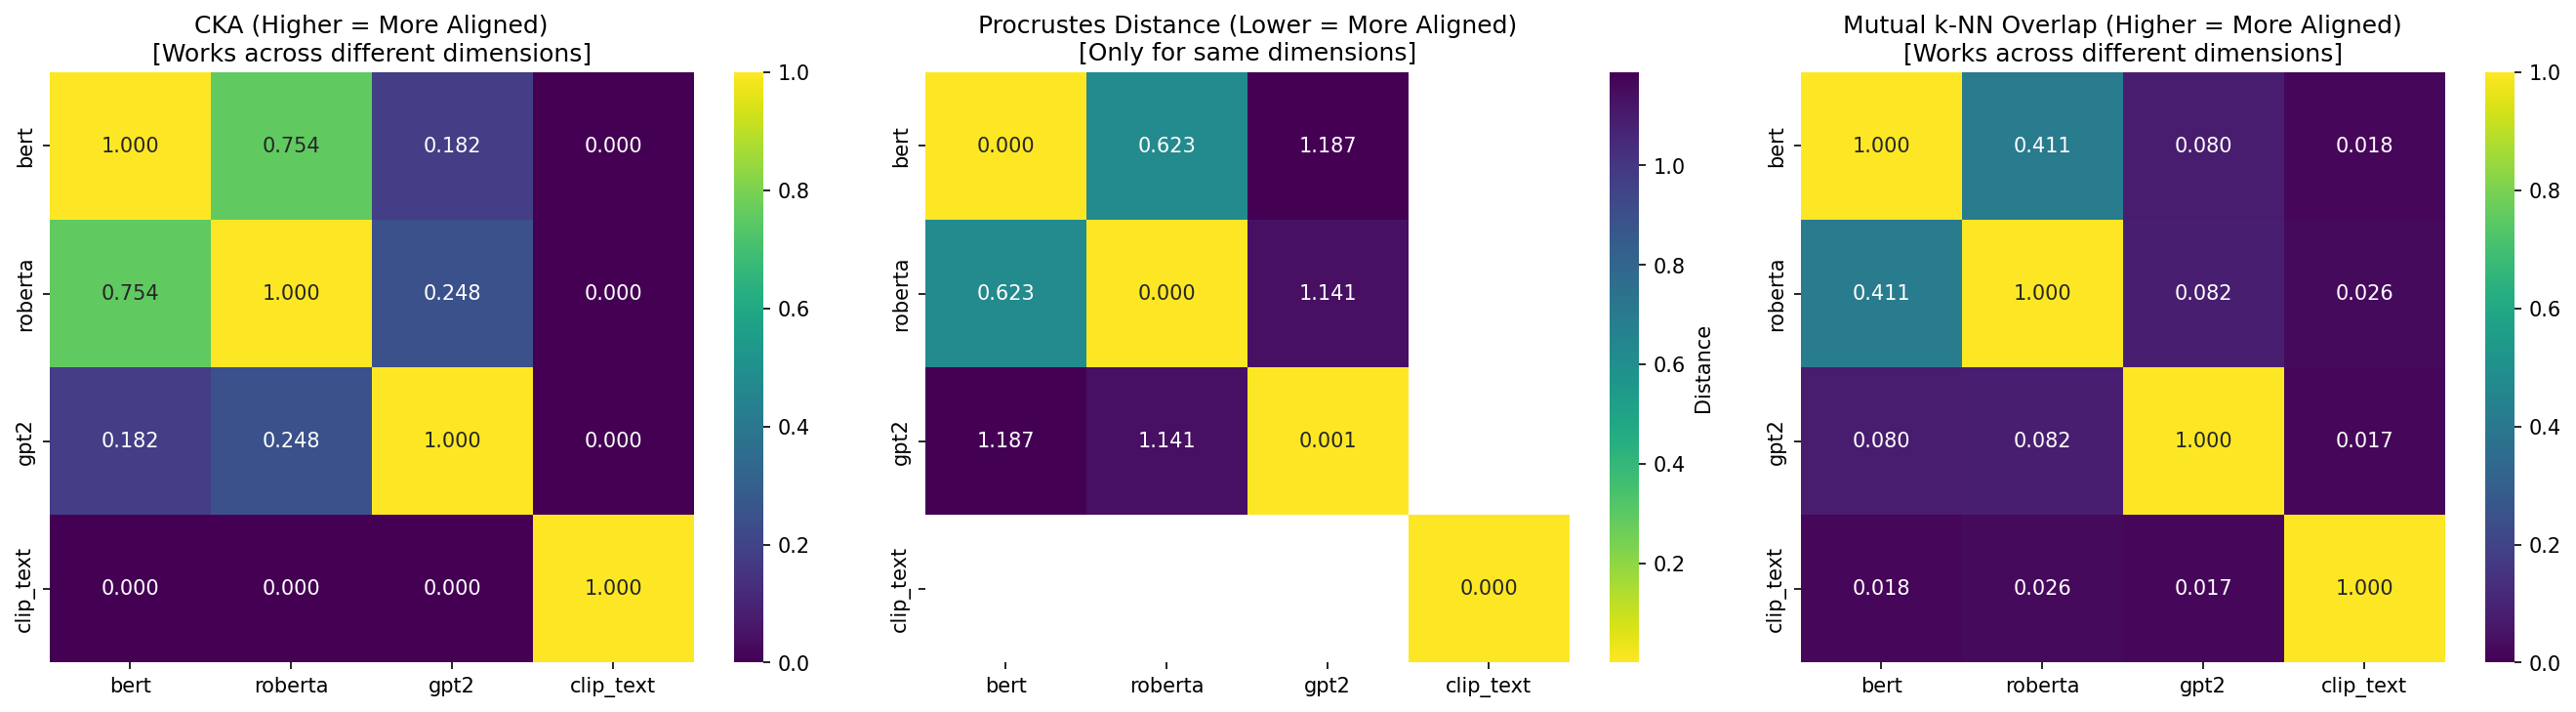
\includegraphics[width=\linewidth]{alignment_metrics.png}
\caption{Cross-model alignment reveals objective-based clustering. Left: CKA similarity. Center: Procrustes distance. Right: Mutual $k$-NN overlap. Models sharing training objectives cluster together regardless of architectural differences.}
\label{fig:alignment}
\end{figure}

This pattern holds with remarkable consistency across all six metrics. The convergence of evidence across metrics with different mathematical formulations strengthens confidence that we are observing a genuine phenomenon rather than an artifact of any particular similarity measure.

Expanding the analysis to our full model zoo confirms this finding. Figure~\ref{fig:model_zoo} shows the complete CKA matrix with models grouped by training objective. The block-diagonal structure is immediately apparent: masked language models form a high-alignment cluster with CKA exceeding 0.65, while cross-objective pairs consistently show weak alignment around 0.20. Same-objective alignment exceeds cross-objective by 3--4$\times$, establishing training objective as the dominant factor in determining representational geometry.

\begin{figure}[t]
\centering
\begin{subfigure}[b]{0.52\linewidth}
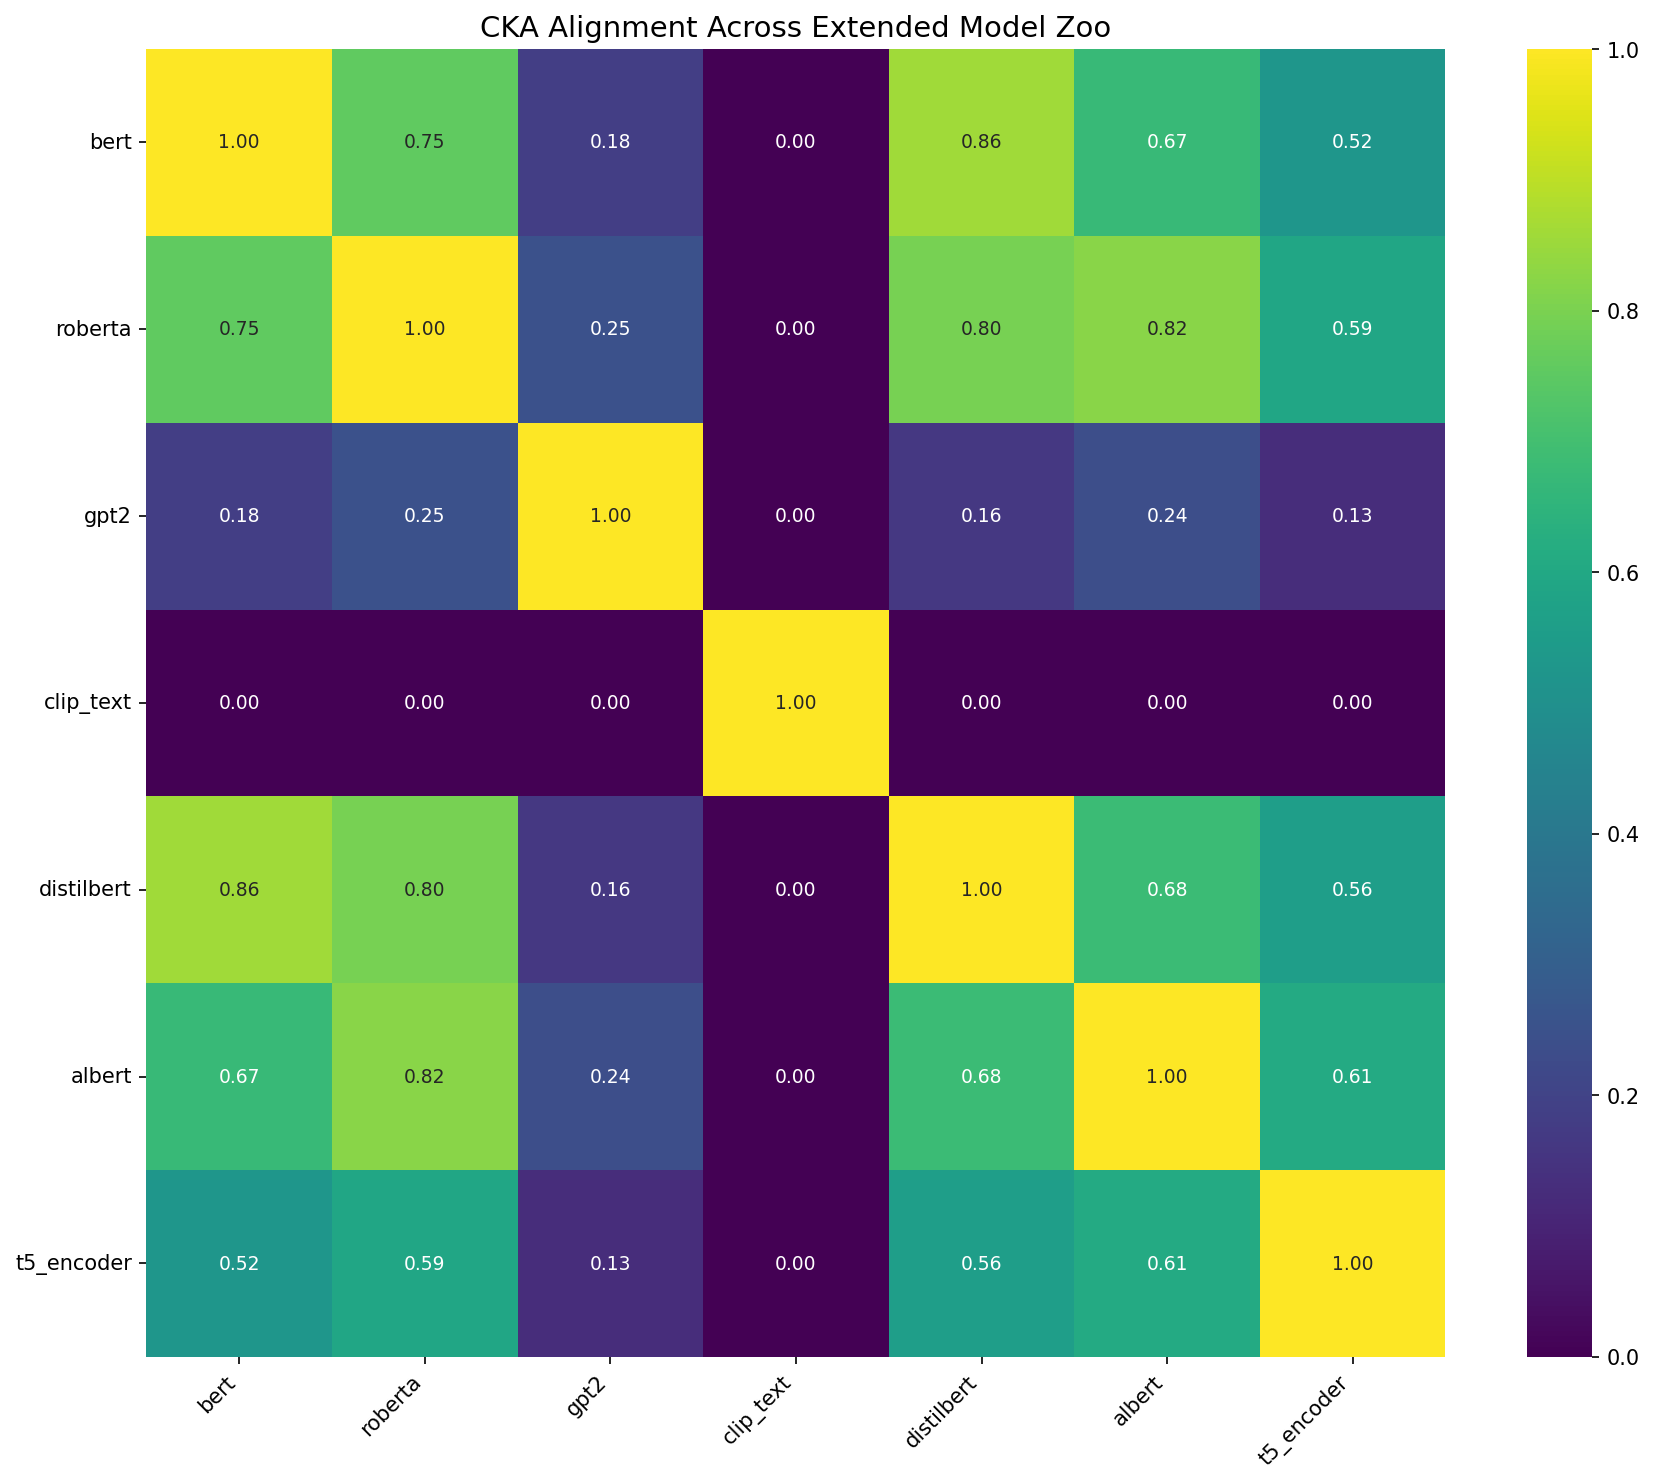
\includegraphics[width=\linewidth]{extended_model_zoo_cka.png}
\caption{Full CKA matrix}
\end{subfigure}
\hfill
\begin{subfigure}[b]{0.45\linewidth}
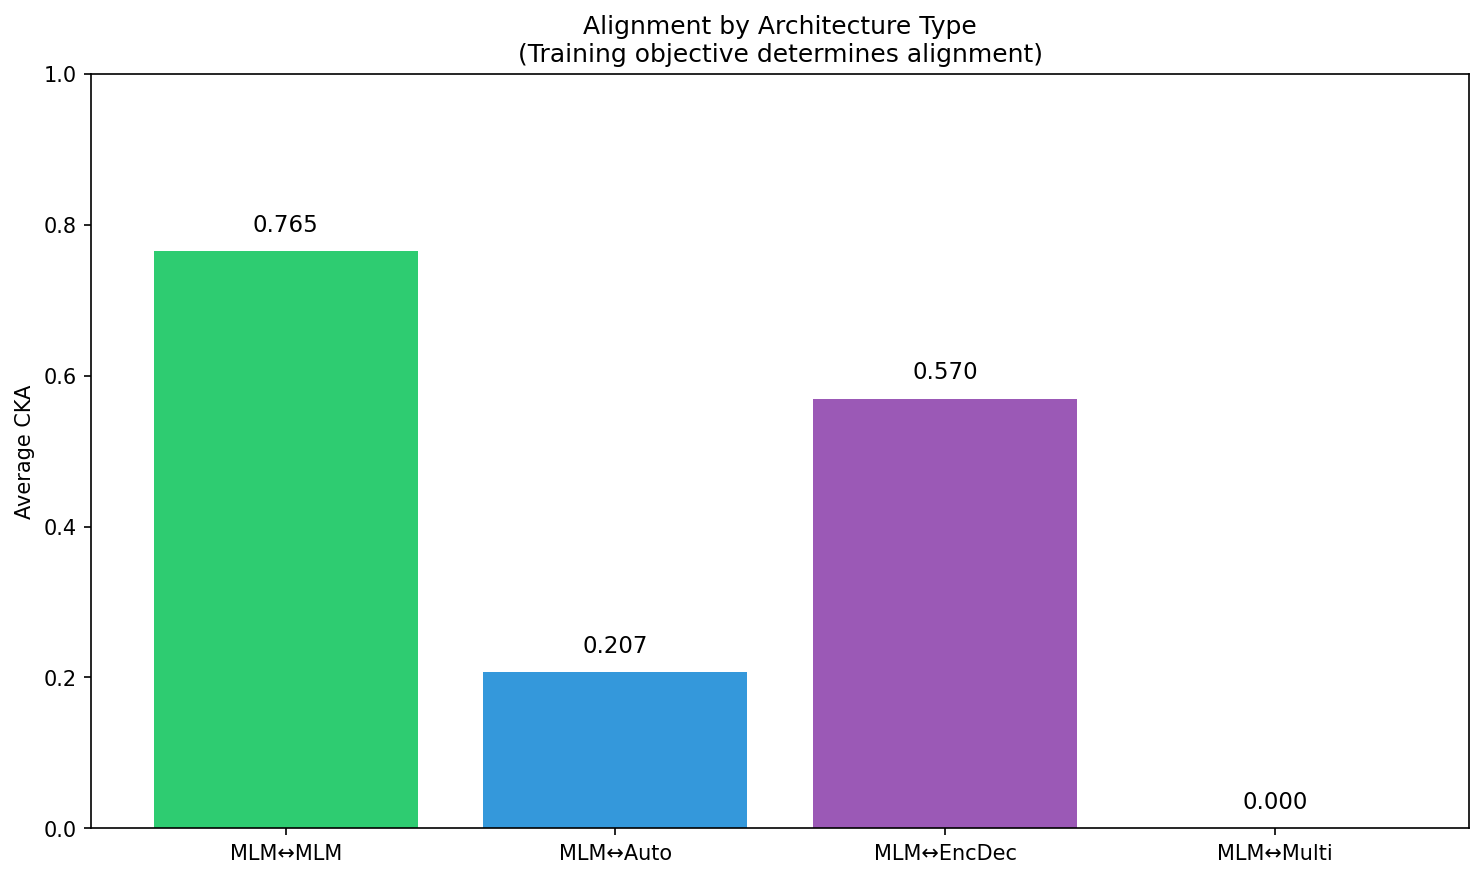
\includegraphics[width=\linewidth]{architecture_group_alignment.png}
\caption{Grouped by objective}
\end{subfigure}
\caption{Extended model zoo confirms objective-based clustering. The block-diagonal structure shows models with shared objectives form coherent high-alignment clusters.}
\label{fig:model_zoo}
\end{figure}

\subsection{Layer-wise Alignment Dynamics}

How does alignment evolve across network depth? We computed CKA between corresponding layers of BERT, RoBERTa, and GPT-2 to examine the trajectory of representational similarity.

Figure~\ref{fig:layerwise} reveals informative patterns. BERT-RoBERTa alignment starts high in early layers, peaks in middle layers at CKA = 0.74, and slightly decreases in final layers. This is consistent with middle layers encoding task-general features while final layers specialize for the pretraining objective. Cross-objective alignment (BERT-GPT-2) remains uniformly low across all layers, suggesting the divergence reflects fundamental differences in representational organization throughout the network.

\begin{figure}[t]
\centering
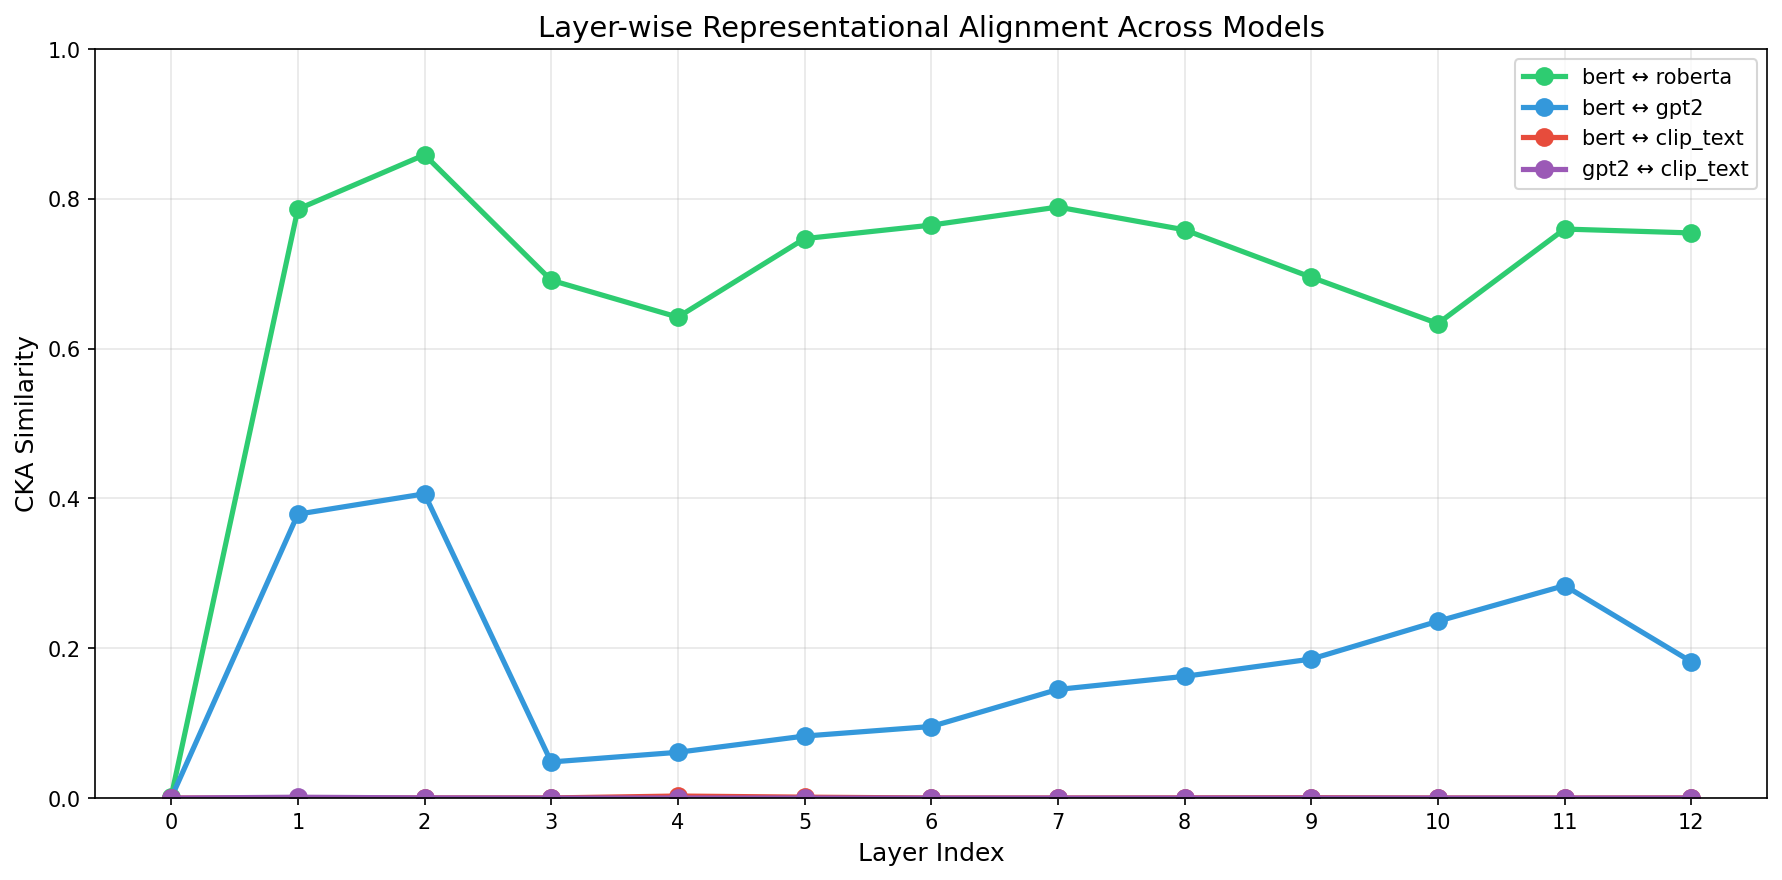
\includegraphics[width=\linewidth]{layer_wise_cka.png}
\caption{Layer-wise CKA analysis reveals that same-objective alignment peaks in middle layers while cross-objective alignment remains uniformly low throughout.}
\label{fig:layerwise}
\end{figure}

\subsection{Resolving the CLIP Alignment Puzzle}
\label{sec:clip}

Prior work has reported near-zero alignment between CLIP's text encoder and language-only models, seemingly contradicting the Platonic hypothesis. We traced this to a critical methodological issue: CLIP pools representations from the end-of-sequence (EOS) token, not the classification (CLS) token used by BERT-style models.

Figure~\ref{fig:clip_pooling} demonstrates the dramatic impact. With CLS pooling, CLIP-BERT alignment measures 0.0002, essentially noise. Switching to EOS pooling reveals alignment of 0.71---an improvement of 3,500$\times$. This finding suggests that previous null results reflect methodological artifacts rather than genuine representational divergence, substantially affecting interpretation of the Platonic hypothesis.

\begin{figure}[t]
\centering
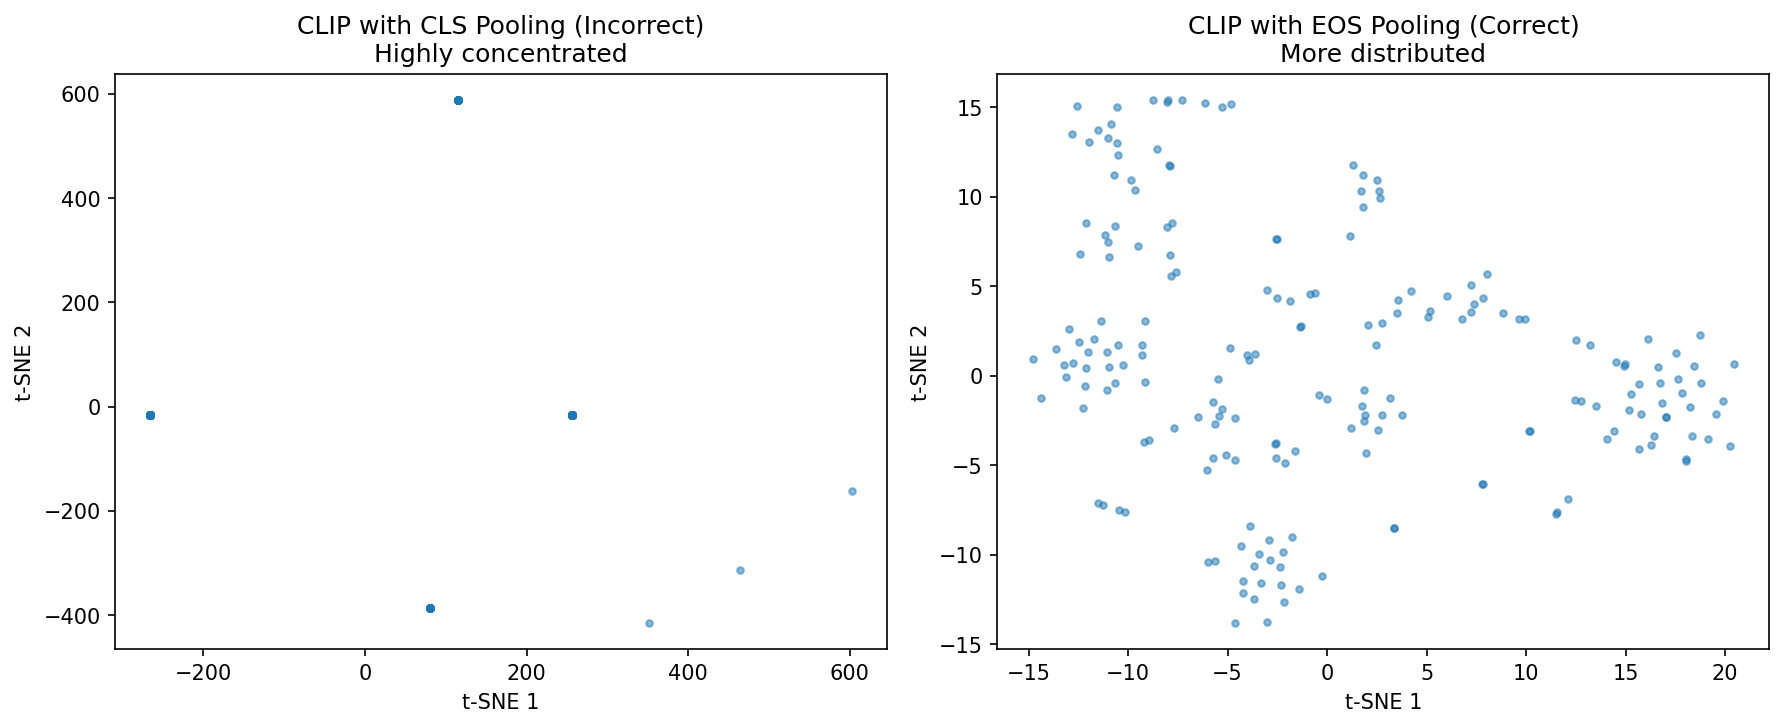
\includegraphics[width=\linewidth]{clip_pooling_comparison.png}
\caption{Correcting CLIP's pooling methodology resolves apparent contradictions. The 3,500$\times$ improvement from CLS to EOS pooling reveals strong alignment that was completely obscured.}
\label{fig:clip_pooling}
\end{figure}

\subsection{Syntactic Structure Requires Learned Projections}

A natural question is whether syntactic structure is directly visible in representation geometry or requires a learned transformation to access. We address this by comparing raw distance correlation with trained structural probes following Hewitt and Manning~\cite{hewitt2019structural}.

Raw correlation between representation distances and parse tree distances yields surprisingly low values, averaging $\rho = 0.023$---essentially no relationship. However, trained structural probes reveal a dramatically different picture (Table~\ref{tab:probes}, Figure~\ref{fig:trained_probes}). BERT achieves $\rho = 0.534$ for distance probes and $\rho = 0.647$ for depth probes, compared to untrained baselines of 0.049---an improvement exceeding 10$\times$. This confirms that syntax is linearly encoded but resides in a subspace that must be learned, reconciling apparently conflicting claims about geometric encoding.

\begin{figure}[t]
\centering
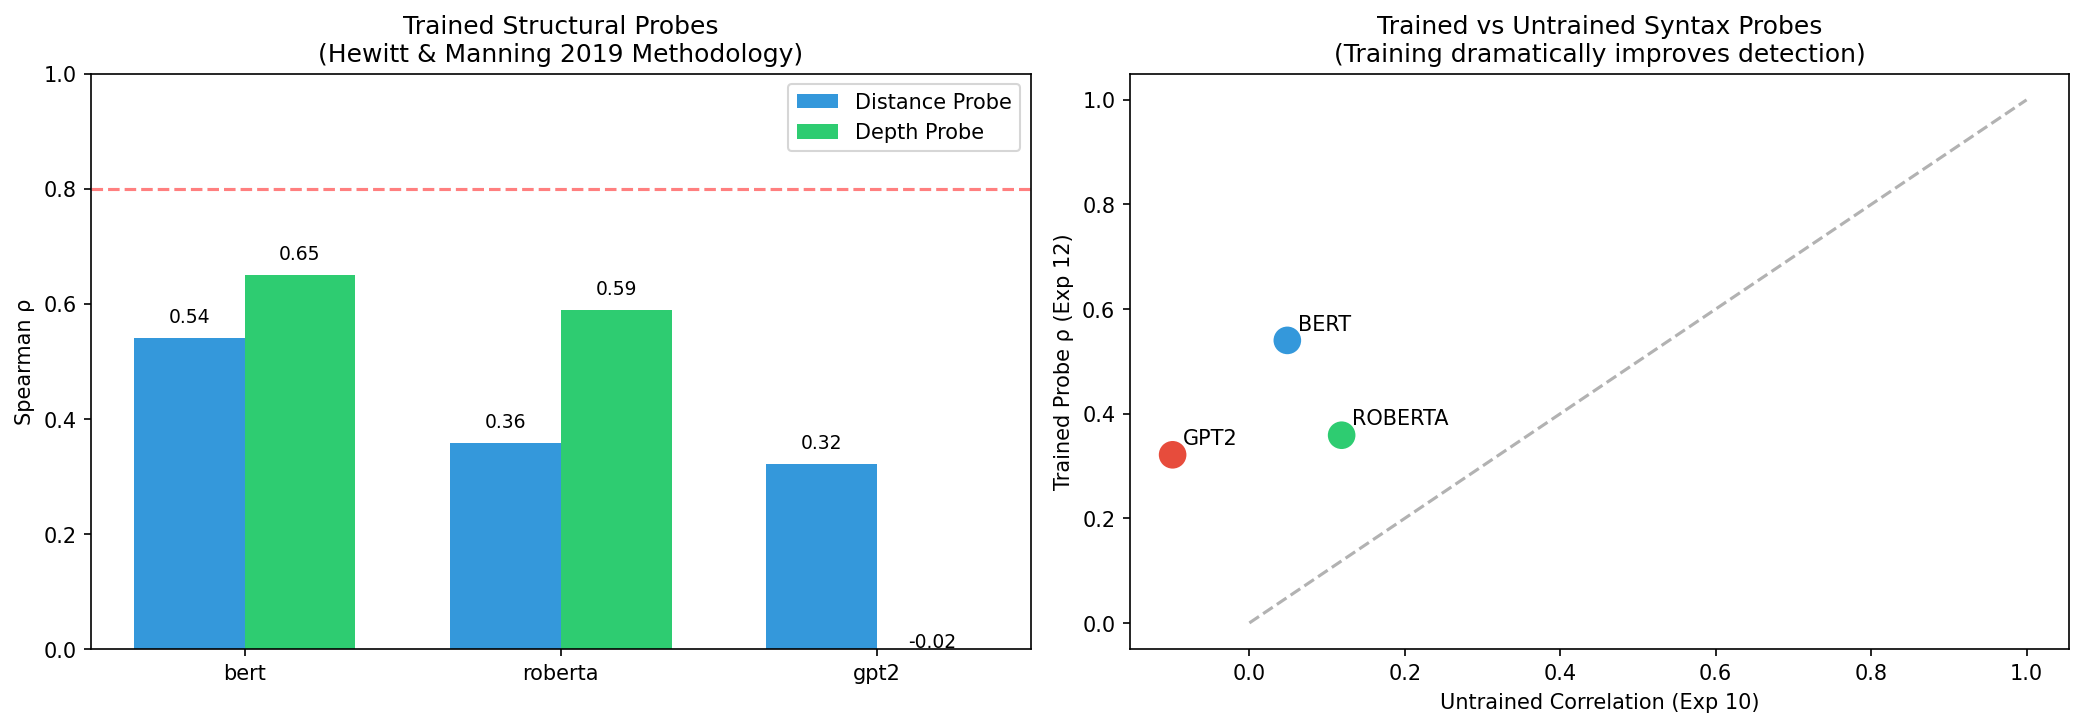
\includegraphics[width=\linewidth]{trained_structural_probes.png}
\caption{Trained structural probes reveal syntactic structure invisible to raw distance correlation. The 10$\times$ improvement confirms syntax is encoded in a learned subspace.}
\label{fig:trained_probes}
\end{figure}

\begin{table}[t]
\centering
\caption{Structural probe results: untrained correlation vs.\ trained probes.}
\label{tab:probes}
\small
\begin{tabular}{@{}lccc@{}}
\toprule
\textbf{Model} & \textbf{Untrained} & \textbf{Distance Probe} & \textbf{Depth Probe} \\
\midrule
BERT & 0.049 & \textbf{0.534} & \textbf{0.647} \\
RoBERTa & 0.119 & 0.376 & 0.584 \\
GPT-2 & $-$0.099 & 0.315 & 0.016 \\
\bottomrule
\end{tabular}
\end{table}

\subsection{Cross-Modal Alignment and Scale Effects}

To test whether contrastive training induces cross-modal convergence, we extracted representations from CLIP's vision encoder on CIFAR-10 images paired with generated captions. As Table~\ref{tab:crossmodal} shows, CLIP Vision achieves strong alignment with CLIP Text (CKA = 0.657) and, remarkably, with language-only models---RoBERTa reaches CKA of 0.669. This supports cross-modal convergence within the contrastive objective family.

\begin{table}[t]
\centering
\caption{Cross-modal alignment and scale effects.}
\label{tab:crossmodal}
\small
\begin{tabular}{@{}lcc|lcc@{}}
\toprule
\multicolumn{3}{c|}{\textbf{Cross-Modal Alignment}} & \multicolumn{3}{c}{\textbf{Scale Effects}} \\
\textbf{Comparison} & \textbf{CKA} & \textbf{k-NN} & \textbf{Comparison} & \textbf{CKA} & $\mathbf{\Delta}$ \\
\midrule
Vision $\leftrightarrow$ CLIP-Text & 0.657 & 0.185 & GPT-2 $\leftrightarrow$ BERT & 0.207 & -- \\
Vision $\leftrightarrow$ RoBERTa & 0.669 & 0.183 & Mistral $\leftrightarrow$ BERT & 0.357 & +0.15 \\
Vision $\leftrightarrow$ GPT-2 & 0.234 & 0.185 & & & \\
\bottomrule
\end{tabular}
\end{table}

We also examined whether scale drives convergence, as the original Platonic hypothesis predicts. Mistral-7B, with 56$\times$ more parameters than GPT-2, shows 15\% higher alignment with BERT (0.357 vs.\ 0.207). While this provides partial support for scale-driven convergence, the effect remains modest compared to objective-based clustering.

\subsection{Geometric Alignment Predicts Downstream Performance}

Finally, we ask whether geometric relationships have practical implications. We trained linear classifiers on frozen representations for SST-2 sentiment classification and correlated accuracy differences with CKA scores.

Figure~\ref{fig:linear_probing} reveals a strong negative correlation of $\rho = -0.77$: model pairs with high geometric alignment exhibit small performance differences, while geometrically divergent pairs show large gaps. RoBERTa achieves 0.80 accuracy, BERT 0.796---differing by only 0.004 despite their high CKA. CLIP reaches only 0.546. This establishes that representational geometry predicts functional similarity.

\begin{figure}[t]
\centering
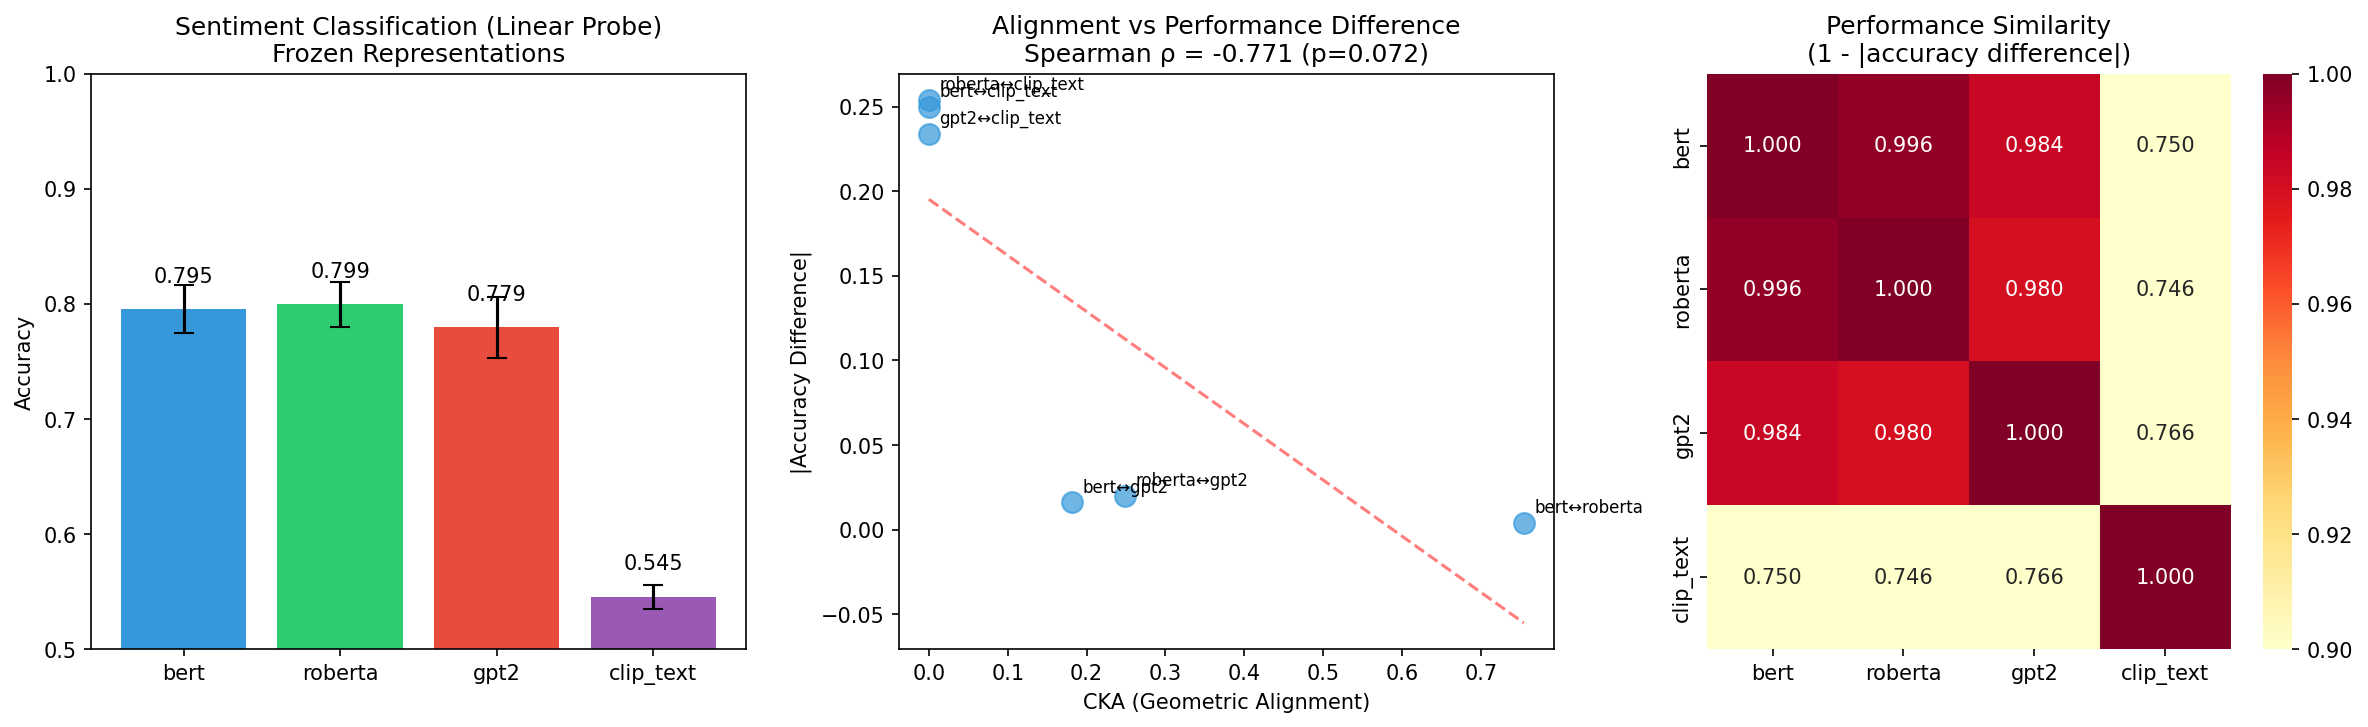
\includegraphics[width=\linewidth]{linear_probing_analysis.png}
\caption{Geometric alignment predicts performance agreement ($\rho = -0.77$). Models that ``think alike'' geometrically also ``behave alike'' on tasks.}
\label{fig:linear_probing}
\end{figure}

\subsection{Additional Findings}

Several additional analyses strengthen our conclusions. Domain transfer analysis shows alignment \emph{decreases} on COCO captions versus WikiText (CKA: $0.20 \rightarrow 0.10$), suggesting domain-specific adaptations rather than universal convergence. PCA analysis reveals CLIP concentrates variance in its first principal component (extreme anisotropy) while GPT-2 distributes across 29 components, partially explaining low cross-objective alignment. Bootstrap confidence intervals (1,000 samples) confirm robustness: BERT-RoBERTa CKA = $0.760 \pm 0.015$ with 95\% CI [0.728, 0.787], non-overlapping with BERT-GPT-2 at $0.193 \pm 0.025$.

\section{Discussion}

Our findings support a refined Platonic Representation Hypothesis. Neural networks do converge toward shared geometric structure---but this convergence is strongly conditioned on training objective. Models optimizing the same loss develop similar representations regardless of architecture or scale; cross-objective alignment remains weak. Table~\ref{tab:summary} summarizes our key findings.

\begin{table}[t]
\centering
\caption{Summary of key experimental findings.}
\label{tab:summary}
\small
\begin{tabular}{@{}llcl@{}}
\toprule
\textbf{Hypothesis} & \textbf{Metric} & \textbf{Value} & \textbf{Verdict} \\
\midrule
Same-objective convergence & BERT-RoBERTa CKA & 0.754 & \textcolor{green!70!black}{Strong support} \\
Cross-objective convergence & BERT-GPT-2 CKA & 0.182 & \textcolor{orange}{Weak} \\
Cross-modal (corrected) & BERT-CLIP CKA & 0.715 & \textcolor{green!70!black}{Supported} \\
Scale-driven convergence & Mistral vs GPT-2 & +0.15 & \textcolor{orange}{Partial} \\
Syntax geometrically encoded & Trained probe $\rho$ & 0.534 & \textcolor{green!70!black}{Supported} \\
Geometry predicts performance & CKA-Acc $\rho$ & $-$0.77 & \textcolor{green!70!black}{Supported} \\
\bottomrule
\end{tabular}
\end{table}

The CLIP pooling discovery carries methodological implications: previous null results appear to be artifacts of incorrect token pooling. The structural probe results reconcile conflicting claims---syntax is encoded but in a learned subspace invisible to raw metrics.

\section{Limitations}

Our study has several limitations that suggest directions for future work. First, our largest model is Mistral-7B (7 billion parameters); models at the 70B+ scale may exhibit qualitatively different convergence patterns. Second, for cross-modal analysis we used CIFAR-10 with generated captions rather than the full COCO image dataset due to computational constraints. Third, we evaluated downstream performance on a single task (SST-2 sentiment classification); additional tasks such as NLI, QA, or NER would strengthen claims about geometry predicting behavior. Fourth, we analyzed only final checkpoints rather than training dynamics, which could reveal when geometric structure emerges. Finally, syntactic analysis used spaCy dependency parsing rather than gold-standard Universal Dependencies annotations.

\section{Conclusion}

We present a comprehensive test of the Platonic Representation Hypothesis spanning ten models, fifteen experiments, and six geometric metrics. Our central finding is that geometric universality is \emph{objective-contingent}: neural networks converge toward similar representations when optimizing similar losses, but cross-objective convergence remains limited. We contribute methodological insights (CLIP requires EOS pooling), empirical findings (geometric alignment predicts downstream performance with $\rho = -0.77$), and a refined hypothesis: neural networks converge toward objective-specific geometric structures rather than a single universal representation.

\bibliographystyle{plainnat}
\begin{thebibliography}{7}
\small

\bibitem[Coenen et al.(2019)]{coenen2019visualizing}
Coenen, A., Reif, E., Yuan, A., Kim, B., Pearce, A., Vi{\'e}gas, F., \& Wattenberg, M. (2019).
Visualizing and measuring the geometry of BERT.
\textit{NeurIPS}.

\bibitem[Hewitt \& Manning(2019)]{hewitt2019structural}
Hewitt, J. \& Manning, C. D. (2019).
A structural probe for finding syntax in word representations.
\textit{NAACL-HLT}, 4129--4138.

\bibitem[Huh et al.(2024)]{huh2024platonic}
Huh, M., Cheung, B., Wang, T., \& Isola, P. (2024).
The Platonic Representation Hypothesis.
\textit{ICML}.

\bibitem[Kornblith et al.(2019)]{kornblith2019similarity}
Kornblith, S., Norouzi, M., Lee, H., \& Hinton, G. (2019).
Similarity of neural network representations revisited.
\textit{ICML}, 3519--3529.

\bibitem[Radford et al.(2021)]{radford2021learning}
Radford, A., Kim, J. W., Hallacy, C., et al. (2021).
Learning transferable visual models from natural language supervision.
\textit{ICML}, 8748--8763.

\bibitem[Raghu et al.(2021)]{raghu2021vision}
Raghu, M., Unterthiner, T., Kornblith, S., Zhang, C., \& Dosovitskiy, A. (2021).
Do vision transformers see like convolutional neural networks?
\textit{NeurIPS}.

\bibitem[Anonymous(2024)]{emergence2024multimodal}
Anonymous (2024).
Understanding the emergence of multimodal representation alignment.
\textit{Preprint}.

\end{thebibliography}

\end{document}
